\documentclass[a4paper, 11pt]{extarticle}
% \usepackage{fontspec}

% ==================================================

% document parameters
% \usepackage[spanish]{babel}
\usepackage[english]{babel}
\usepackage[margin = 1in]{geometry}
\usepackage{subcaption}
\usepackage{algorithm}
\usepackage{algpseudocode}
% ==================================================

% Packages for math
\usepackage{mathrsfs}
\usepackage{amsfonts}
\usepackage{amsmath}
\numberwithin{equation}{subsection}
\usepackage{amsthm}
\usepackage{amssymb}
\usepackage{physics}
\usepackage{dsfont}
\usepackage{esint}
\usepackage{tikz}
\usepackage{tikz-3dplot}
\usetikzlibrary{positioning, arrows.meta, backgrounds, fit, calc}

% ==================================================

% Packages for writing
\usepackage{enumerate}
\usepackage[shortlabels]{enumitem}
\usepackage{framed}
\usepackage[utf8]{inputenc}
\usepackage{csquotes}


% ==================================================

% Miscellaneous packages
\usepackage{float}
\usepackage{tabularx}
\usepackage{multicol}
\usepackage{subcaption}
\usepackage{caption}
\captionsetup{format = hang, margin = 10pt, font = small, labelfont = bf}

% Citation
\usepackage[numbers, square]{natbib}

% Hyperlinks setup
\usepackage{hyperref}
\usepackage{cleveref}
\usepackage{listings}
\usepackage{etoolbox}
\usepackage{xcolor}
\usepackage{quoting}
\usepackage{changepage} % for adjustwidth

\newenvironment{fancyquote}[1][]
{\begin{adjustwidth}{2em}{2em}%
		\itshape
		\ifstrempty{#1}{}{---\ #1\\[1ex]}}
	{\end{adjustwidth}\vspace{1em}}


\lstset{
    language=Python,
    basicstyle=\ttfamily\footnotesize,
    keywordstyle=\color{blue},
    commentstyle=\color{gray},
    stringstyle=\color{red},
    breaklines=true,
    numbers=left,
    numberstyle=\tiny,
    stepnumber=1,
    numbersep=5pt,
    frame=single,
    captionpos=b,
    tabsize=4,
    showstringspaces=false,
}

\definecolor{links}{rgb}{0.36,0.54,0.66}
\hypersetup{
    colorlinks = false,
    linkcolor = red,
    urlcolor = blue,
    citecolor = blue,
    filecolor = blue,
    pdfauthor = {Author},
    pdftitle = {Title},
    pdfsubject = {subject},
    pdfborder = {0 0 1},
    linkbordercolor = {1 0 0},
    citebordercolor = {1 0 0},
    urlbordercolor  = {1 0 0},
    pdfkeywords = {one, two},
    pdfproducer = {LaTeX},
    pdfcreator = {pdfLaTeX},
   }

\theoremstyle{plain}
\newtheorem{theorem}{Theorem}[section]
\newtheorem{lemma}[theorem]{Lemma}
\newtheorem{proposition}[theorem]{Proposition}
\newtheorem{corollary}{Corollary}

\theoremstyle{definition}
\newtheorem{definition}{Definition}[section]
\newtheorem{axiom}{Axiom}[section]
\newtheorem{conjecture}{Conjecture}[section]
%\newtheorem{example}{Example}[section]

\theoremstyle{remark}
\newtheorem{remark}{Remark}
\newtheorem*{note}{Note}

\usepackage{mdframed}
% Define colors
\definecolor{formalshade}{rgb}{0.95,0.95,1} % Light blue background
\definecolor{darkblue}{rgb}{0.0, 0.0, 0.55} % Border color
\newmdenv[
  leftmargin=4pt,
  rightmargin=4pt,
  backgroundcolor=formalshade,
  linecolor=darkblue,
  linewidth=2pt,
  roundcorner=4pt,
  innerleftmargin=6pt,
  innerrightmargin=6pt,
  innertopmargin=6pt,
  innerbottommargin=6pt,
  skipabove=6pt,
  skipbelow=6pt,
  nobreak=true, % Allows spanning pages
]{formal}

\usepackage{booktabs}  % For \toprule, \midrule, \bottomrule
\usepackage{array}     % For improved table formatting

\newcommand{\notimplies}{\;\not\!\!\!\implies}

%%%%%%%%%%%%%%%%%%%%%%%%% HEADER AND FOOTER
\usepackage{fancyhdr}
\pagestyle{fancy}
\fancypagestyle{plain}
\fancyhf{}
\lhead{ASF}
\rhead{DBL SP25}

% --- Basic commands ---
%   Euler's constant
\newcommand{\eu}{\mathrm{e}}

%   Imaginary unit
\newcommand{\im}{\mathrm{i}}

%   Sexagesimal degree symbol
\newcommand{\grado}{\,^{\circ}}

% --- Comandos para álgebra lineal ---
% Matrix transpose
\newcommand{\transpose}[1]{{#1}^{\mathsf{T}}}

%%% Comandos para cálculo
%   Definite integral from -\infty to +\infty
\newcommand{\Int}{\int\limits_{-\infty}^{\infty}}

%   Indefinite integral
\newcommand{\rint}[2]{\int{#1}\dd{#2}}

%  Definite integral
\newcommand{\Rint}[4]{\int\limits_{#1}^{#2}{#3}\dd{#4}}

%   Dot product symbol (use the command \bigcdot)
\makeatletter
\newcommand*\bigcdot{\mathpalette\bigcdot@{.5}}
\newcommand*\bigcdot@[2]{\mathbin{\vcenter{\hbox{\scalebox{#2}{$\m@th#1\bullet$}}}}}
\makeatother

%   Hamiltonian
\newcommand{\Ham}{\hat{\mathcal{H}}}

%   Trace
\renewcommand{\Tr}{\mathrm{Tr}}

% Christoffel symbol of the second kind
\newcommand{\christoffelsecond}[4]{\dfrac{1}{2}g^{#3 #4}(\partial_{#1} g_{#2 #4} + \partial_{#2} g_{#1 #4} - \partial_{#4} g_{#1 #2})}

% Riemann curvature tensor
\newcommand{\riemanncurvature}[5]{\partial_{#3} \Gamma_{#4 #2}^{#1} - \partial_{#4} \Gamma_{#3 #2}^{#1} + \Gamma_{#3 #5}^{#1} \Gamma_{#4 #2}^{#5} - \Gamma_{#4 #5}^{#1} \Gamma_{#3 #2}^{#5}}

% Covariant Riemann curvature tensor
\newcommand{\covariantriemanncurvature}[5]{g_{#1 #5} R^{#5}{}_{#2 #3 #4}}

% Ricci tensor
\newcommand{\riccitensor}[5]{g_{#1 #5} R^{#5}{}_{#2 #3 #4}}

% \renewcommand{\familydefault}{\sfdefault}

% Boldface unit vector with a hat
\newcommand{\uv}[1]{\mathbf{\hat{#1}}}

\newcommand{\ep}{\varepsilon}

\DeclareMathOperator{\sgn}{sgn}

\usepackage{titlesec}
\usepackage[many]{tcolorbox}

% Adjust spacing after the chapter title
\titlespacing*{\chapter}{0cm}{-2.0cm}{0.50cm}
\titlespacing*{\section}{0cm}{0.50cm}{0.25cm}

% Indent 
\setlength{\parindent}{0pt}
\setlength{\parskip}{1ex}

% --- Theorems, lemma, corollary, postulate, definition ---
% \numberwithin{equation}{section}
\tcbuselibrary{skins, breakable,theorems}
\newtcbtheorem[]{problem}{Problem}%
    {enhanced,
    colback = black!5, %white,
    colbacktitle = black!5,
    coltitle = black,
    boxrule = 0pt,
    frame hidden,
    borderline west = {0.5mm}{0.0mm}{black},
    fonttitle = \bfseries\sffamily,
    breakable,
    before skip = 3ex,
    after skip = 3ex
}{problem}
\makeatletter
\let\example\relax
\makeatother
% Forcefully undefine \example (this is sometimes needed if it’s already defined)
\makeatletter
\let\example\relax
\makeatother

% Now define the 'example' environment using tcolorbox theorem style:
\newtcbtheorem[]{example}{Example}%
  {enhanced,
   colback = black!5, % background color
   colbacktitle = black!5, % title background color
   coltitle = black, % title text color
   boxrule = 0pt, % no box border
   frame hidden,
   borderline west = {0.5mm}{0.0mm}{black},
   fonttitle = \bfseries\sffamily,
   breakable,
   before skip = 3ex,
   after skip = 3ex
  }{example}
\newcommand{\vphi}{\varphi}

% --- You can define your own color box. Just copy the previous \newtcbtheorm definition and use the colors of yout liking and the title you want to use.

\newcommand{\bb}{\mathbb}
\usepackage[bottom]{footmisc}
%% Commands for PSET6

\begin{document}
	
	\begin{center}
		\begin{huge}
			{\textbf{\texttt{catLC}: Multiscale Categorical Field Theory for Liquid Crystals [\texttt{WIP, v0.2}]}}\\[2ex]
		\end{huge}
		
		\begin{Large}
			by Alejandro Soto Franco\footnote{\texttt{asoto12@jhu.edu, sotofranco.math@gmail.com}}, last updated \today
		\end{Large}
	\end{center}
	
	\thispagestyle{empty}
	
	\tableofcontents
	
	\newpage
	
	\section{Introduction}
	
	Information underlies every physical model. Whether encoded in molecular configurations, order parameter fields, or large-scale defect networks, nature computes its behavior through structured data. As Deutsch explores across various constants for universe iterations in his \emph{The Fabric of Reality} \cite{deutsch1997fabric}, information is encoded in regular patterns that can be physically realized through the identification of invariances up to a particular resolution scale. In liquid crystal theory, this viewpoint connects phenomena across scales, from microscopic interactions to macroscopic defect networks, as detailed in \cite{degennes1993physics, cardy1996scaling, ma1976modern}.
	
	A powerful tool for understanding multiscale phenomena is the \textbf{renormalization group (RG)}. RG flow describes how system parameters evolve as one “zooms out” and coarse-grains microscopic details. In the context of liquid crystals, local molecular interactions are aggregated into effective mesoscopic order parameters and further into macroscopic defect configurations. This coarse-graining procedure not only reveals fixed points corresponding to phase transitions but also uncovers the propagation of local fluctuations across scales.
	
	Inspired by the structural insights of category theory \cite{maclane1971categories, spivak2014category} and by developments in topological quantum field theory \cite{atiyah1988topological, segal2004definition, freed1995chern}, we propose a \emph{multiscale categorical field theory for liquid crystals}. In this framework:
	\begin{itemize}
		\item \textbf{Objects} represent complete informational states at various scales—from microscopic molecular configurations through mesoscopic \(Q\)-tensor fields to macroscopic defect networks \cite{degennes1993physics}.
		\item \textbf{Morphisms} encode the dynamical or topological transitions between these states, including the RG transformations that systematically integrate out degrees of freedom \cite{cardy1996scaling, ma1976modern}.
		\item \textbf{Functors} serve to relate and translate information between different levels of description, much like RG maps relate theories at distinct scales \cite{baez2011rosetta, abramsky2004categorical}.
	\end{itemize}
	
	Moreover, our approach establishes links with higher gauge theories \cite{baez2007higher} and categorical semantics in quantum protocols \cite{selinger2007dagger, abramsky2004categorical}, emphasizing the universality of compositional principles across physics.
	
	\section{Categorical Renormalization Group Flows}
	
	Consider a microscopic state \(A\) of a liquid crystal system, characterized by detailed molecular configurations. The RG flow defines a map 
	\[
	R: A \to B,
	\]
	where \(B\) represents a mesoscopic state described by an effective \(Q\)-tensor field. Repeated application of the RG transformation leads to a sequence of states
	\[
	A \xrightarrow{R_1} B \xrightarrow{R_2} C \xrightarrow{R_3} \cdots,
	\]
	with each \(R_i\) acting as a morphism in the category \(\mathcal{C}\) of informational states. The composition
	\[
	R_{n} \circ \cdots \circ R_2 \circ R_1
	\]
	then represents the full RG flow from the microscopic to the macroscopic scale. By the associativity of morphism composition \cite{maclane1971categories}, this overall transformation is well-defined regardless of the grouping of intermediate steps.
	
	\subsection{Functoriality and structure preserving mappings}
	
	Within our framework, the RG transformation is treated as a functor:
	\[
	\mathcal{R}: \mathcal{C}_{\text{micro}} \to \mathcal{C}_{\text{meso}},
	\]
	mapping microscopic theories to effective mesoscopic descriptions. This functor satisfies:
	\begin{enumerate}[label=(\alph*)]
		\item For every object \(A \in \mathcal{C}_{\text{micro}}\), the image \(\mathcal{R}(A)\) is an object in \(\mathcal{C}_{\text{meso}}\) that encapsulates coarse-grained information \cite{spivak2014category}.
		\item For every morphism \(f: A \to B\) in \(\mathcal{C}_{\text{micro}}\), the functor assigns a morphism \(\mathcal{R}(f): \mathcal{R}(A) \to \mathcal{R}(B)\) such that
		\[
		\mathcal{R}(g \circ f) = \mathcal{R}(g) \circ \mathcal{R}(f),
		\]
		thereby preserving the compositional structure \cite{atiyah1988topological, segal2004definition}.
	\end{enumerate}
	
	This functorial view parallels constructions in topological quantum field theory \cite{freed1995chern} and higher gauge theory \cite{baez2007higher}, ensuring that the underlying informational structure is maintained across scales.
	
	\subsection{Nematic order and RG in field space}
	
	Nematic liquid crystals are described by a headless unit vector field (director field) \( \mathbf{n}(x) \sim -\mathbf{n}(x) \), or equivalently by a symmetric, traceless \(Q\)-tensor field \( Q_{ij}(x) \). This tensor field encodes both the degree of orientational order and its anisotropy \cite{degennes1993physics}.

	Under coarse-graining, local fluctuations in the director field are averaged out to produce a smoothed \(Q\)-field. The renormalization group transformation at each scale acts by:
	\[
	Q^{(k+1)}(x) = \int_{B_\epsilon(x)} K_\epsilon(x,y) Q^{(k)}(y) \, d\mathrm{vol}_{g}(y),
	\]
	where \(K_\epsilon\) is a smoothing kernel localized over scale \(\epsilon\). This defines a geometric flow in field space, compatible with the categorical flow on configurations.

	Defects such as disclinations manifest as topological singularities in the field configuration and are preserved or annihilated under RG evolution depending on their energy cost and scale relevance.

	Thus, the object class in \(\mathcal{C}_{\text{meso}}\) includes \( (M^d, Q) \) pairs modulo topological equivalence under gauge group \(G\), with morphisms describing admissible transitions under geometric and RG flows.

	\subsection{Example of RG flow computation with Rust}
	
	The RG transformation can be decomposed into two primary operations:
	\begin{enumerate}[label=(\arabic*)]
		\item \textbf{Local Averaging (Map Operation):} For each local region \(R\) in the microscopic state, compute an order parameter \(q_R\) that summarizes the local configuration. This step corresponds to integrating out high-frequency modes \cite{degennes1993physics}.
		\item \textbf{Aggregation (Reduce Operation):} Combine the locally computed order parameters \(q_R\) to form the effective mesoscopic state \(B\) by aggregating local contributions into a global structure \cite{hudak1989conception}.
	\end{enumerate}
	
	Mathematically, if the microscopic state is partitioned into regions \( \{ R_1, R_2, \dots, R_N \} \) with associated order parameters
	\[
	q_{R_i} = \texttt{compute\_order}(R_i),
	\]
	the mesoscopic state is constructed as
	\[
	B = \texttt{aggregate}(\{q_{R_1}, q_{R_2}, \dots, q_{R_N}\}).
	\]
	
	An iterative RG flow is then represented as:
	\[
	A^{(0)} \xrightarrow{R^{(1)}} A^{(1)} \xrightarrow{R^{(2)}} A^{(2)} \xrightarrow{R^{(3)}} \cdots,
	\]
	with convergence toward a fixed point \(A^{(\infty)}\) satisfying
	\[
	R(A^{(\infty)}) \cong A^{(\infty)}.
	\]
	
	The following Rust code illustrates a preliminary implementation of a single RG transformation step. The implementation reflects a functional programming style reminiscent of Haskell \cite{hudak1989conception}:
	
	\begin{lstlisting}[caption={Rust Implementation of a Single RG Transformation Step}]
		#[derive(Debug)]
		struct Region {
			// Microscopic configuration in a local region.
			data: Vec<f64>,
		}
		
		#[derive(Debug)]
		struct MicroscopicState {
			// Collection of local regions.
			regions: Vec<Region>,
		}
		
		#[derive(Debug)]
		struct OrderParameter {
			// Local order parameter computed for a region.
			value: f64,
		}
		
		#[derive(Debug)]
		struct MesoscopicState {
			// Aggregated mesoscopic state.
			order_parameters: Vec<OrderParameter>,
		}
		
		/// Computes the local order parameter for a given region.
		fn compute_order(region: &Region) -> OrderParameter {
			let sum: f64 = region.data.iter().sum();
			let avg = sum / (region.data.len() as f64);
			OrderParameter { value: avg }
		}
		
		/// Aggregates local order parameters into a mesoscopic state.
		fn aggregate(order_parameters: Vec<OrderParameter>) -> MesoscopicState {
			MesoscopicState { order_parameters }
		}
		
		/// Performs a single RG transformation step.
		fn rg_step(microscopic: &MicroscopicState) -> MesoscopicState {
			let order_parameters: Vec<OrderParameter> = microscopic.regions
			.iter()
			.map(|region| compute_order(region)) /// where a lot of the computational work of our lab and its collaborators has been focused
			.collect();
			aggregate(order_parameters)
		}
		
		fn main() {
			let region1 = Region { data: vec![1.0, 2.0, 3.0] };
			let region2 = Region { data: vec![4.0, 5.0, 6.0] };
			let region3 = Region { data: vec![7.0, 8.0, 9.0] };
			let microscopic = MicroscopicState {
				regions: vec![region1, region2, region3],
			};
			let mesoscopic = rg_step(&microscopic);
			println!("Mesoscopic state: {:?}", mesoscopic);
		}
	\end{lstlisting}
	
	\subsection{Curved geometry and stochastic dynamics}
		Beyond standard RG flows, our framework accommodates evolving geometries and stochastic dynamics. Here, the microscopic theories are defined on a high-dimensional manifold \(M\) whose geometry evolves via curvature-driven flows (e.g., mean curvature flow or Ricci flow) \cite{hamilton1982three, grayson1987shortening}. 
	
	To capture stochastic evolution, we introduce Markov chain dynamics governed by a probability kernel \(P\) \cite{levin2009markov}. In this enriched setting, the RG flow functor
	\[
	\mathcal{R}: \mathcal{C}_{\text{micro}}^G \to \mathcal{C}_{\text{meso}}^G,
	\]
	acts as a Markov operator with the following properties:
	\begin{enumerate}[label=(\alph*)]
		\item Each microscopic object \((M, \phi)\) is mapped to an effective mesoscopic object \(\mathcal{R}(M, \phi) = (\widetilde{M}, \widetilde{\phi})\) through geometric smoothing and statistical averaging \cite{e2003multiscale}.
		\item For every morphism \(f: (M, \phi) \to (M', \phi')\) with transition probability \(P\big((M, \phi), (M', \phi')\big)\), the functor assigns a corresponding morphism \(\mathcal{R}(f)\) that preserves the probabilistic structure.
	\end{enumerate}
	
	This approach aligns with methods in topological quantum field theory \cite{atiyah1988topological, guillemin1984symplectic} and provides a robust framework for exploring universality in complex systems. Let $(M^d, g(t))$ be a family of Riemannian manifolds with evolving metric. For Ricci flow:
	\[
	\frac{\partial}{\partial t} g_{ij} (t) = - 2 \mathrm{Ric}_{ij} (t),
	\]
	where $\mathrm{Ric}_{ij}$ is the Ricci curvature tensor associated with $g(t)$. In local coordinates, we compute
	\[
	\mathrm{Ric}_{ij} = \partial_k \Gamma_{ij}^k + \Gamma_{ij}^k \Gamma_{kl}^l - \Gamma_{ik}^l \Gamma_{jl}^k,
	\]
	where the Christoffel symbols are given by
	\[
	\Gamma^{k}_{ij} = \frac{1}{2} g^{kl} (\partial_i g_{jl} + \partial_j g_{il} - \partial_l g_{ij}).
	\]
	
	The evolution of the metric directly alters distances, volumes, and local operator representations, such as the Laplace–Beltrami operator:
	\[
	\Delta_{g(t)} f = \frac{1}{\sqrt{|g(t)|}} \partial_i \left( \sqrt{|g(t)|} \, g^{ij}(t) \, \partial_j f \right),
	\]
	which governs diffusion and heat flow on curved geometries \cite{chow2004ricci, morgan2007ricci}.
	
	To incorporate stochastic dynamics, we model the evolution of field configurations $\phi: M \to \mathbb{R}^n$ using a generator $\mathcal{L}_t$:
	\[
	\mathcal{L}_t = \Delta_{g(t)} + b^i(t,x) \partial_i + V(t,x),
	\]
	where $b^i$ encodes drift and $V$ represents a curvature-coupled potential. The probability distribution $\mu_t$ of such configurations then satisfies a Fokker–Planck equation:
	\[
	\frac{d\mu_t}{dt} = \mathcal{L}_t^* \mu_t.
	\]
	
	Within the enriched categorical setting, the RG functor $
	\mathcal{R}_t: \mathcal{C}_{\mathrm{micro}}^G \to \mathcal{C}_{\mathrm{meso}}^G $ acts on objects $(M, \phi)$ by mapping them to effective mesoscopic configurations:
	\[
	\mathcal{R}_t(M, \phi) = (\widetilde{M}, \widetilde{\phi}),
	\]
	where $\widetilde{M}$ is the evolved manifold under Ricci flow and
	\[
	\widetilde{\phi}(x) = \int_M K_t(x,y) \phi(y) \, d\mathrm{vol}_{g(t)}(y)
	\]
	is the heat-kernel-smoothed field with kernel $K_t(x,y)$.
	
	This construction generalizes stochastic quantization techniques \cite{damgaard1987stochastic}, multiscale coarse-graining via geometric flows \cite{e2003multiscale}, and Bayesian field inference on manifolds \cite{cotter2013bayesian}, providing a robust framework for studying universal behavior in dynamically evolving, curved backgrounds.
	
	\section{Methods}
	
	\subsection{Categorical foundations}
	
	A \emph{category} \(\mathcal{C}\) consists of:
	\begin{enumerate}[label=(\roman*)]
		\item A collection \(\mathrm{Ob}(\mathcal{C})\) of \textbf{objects}, each representing an informational state (e.g., a detailed \(Q\)-tensor field, director configuration, or defect network) \cite{maclane1971categories, spivak2014category}.
		\item For any two objects \(A,B \in \mathrm{Ob}(\mathcal{C})\), a set \(\mathrm{Hom}_{\mathcal{C}}(A,B)\) of \textbf{morphisms} that represent transitions or processes from \(A\) to \(B\) \cite{maclane1971categories}.
		\item A composition law: For any morphisms \(f \in \mathrm{Hom}_{\mathcal{C}}(A,B)\) and \(g \in \mathrm{Hom}_{\mathcal{C}}(B,C)\), the composite morphism \(g\circ f \in \mathrm{Hom}_{\mathcal{C}}(A,C)\) satisfies
		\[
		h\circ (g\circ f) = (h\circ g)\circ f,
		\]
		for all choices of \(f\), \(g\), and \(h\) \cite{maclane1971categories}.
		\item For each object \(A\), an identity morphism \(\mathrm{id}_A\) satisfying
		\[
		f\circ \mathrm{id}_A = f \quad \text{and} \quad \mathrm{id}_B\circ f = f,
		\]
		for every \(f \in \mathrm{Hom}_{\mathcal{C}}(A,B)\).
	\end{enumerate}
	
	This structure is analogous to those found in topological and symplectic categories \cite{weinstein1981symplectic, guillemin1984symplectic}.
	
	\begin{axiom}[Informational Conjecture]
		Every object in \(\mathcal{C}\) is a repository of information. In liquid crystal physics, an object may encode microscopic molecular configurations, mesoscopic \(Q\)-tensor fields, or macroscopic defect networks \cite{degennes1993physics, spivak2014category}.
	\end{axiom}
	
	\begin{remark}
		Morphisms in \(\mathcal{C}\) represent the dynamical or topological transitions between informational states. Their composition mirrors the pure function composition in functional programming \cite{hudak1989conception} and extends naturally to categorical semantics in quantum protocols \cite{abramsky2004categorical, selinger2007dagger}.
	\end{remark}
	
	\begin{theorem}[Associativity of Compositional Transformations]
		For any morphisms \(f: A \to B\), \(g: B \to C\), and \(h: C \to D\) in \(\mathcal{C}\), we have
		\[
		h\circ (g\circ f) = (h\circ g)\circ f.
		\]
	\end{theorem}
	
	\begin{proof}
		This follows directly from the definition of a category \cite{maclane1971categories}.
	\end{proof}
	
	\subsection{Functorial Beris-Edwards model on smooth manifolds}
	
	The Beris–Edwards model describes the hydrodynamic evolution of a nematic liquid crystal via coupled equations for a velocity field \( u^i \) and a \( Q \)-tensor field \( Q_{ij} \). The evolution equation on a Riemannian manifold \( (M^d, g) \) with Levi-Civita connection \( \nabla \) is:
	\[
	(\partial_t + u^k \nabla_k) Q_{ij} - S_{ij} = \Gamma H_{ij},
	\]
	where \( \Gamma \) is a collective rotational viscosity, \( H_{ij} = - \frac{\delta F}{\delta Q_{ij}} \) is the molecular field derived from the Landau–de Gennes free energy \( F[Q] \), and \( S_{ij} \) encodes the response to velocity gradients:
	\[
	S_{ij} = (\xi D_{ik} + \Omega_{ik})(Q_{kj} + \tfrac{1}{d} \delta_{kj}) + (Q_{ik} + \tfrac{1}{d} \delta_{ik})(\xi D_{kj} - \Omega_{kj}) - 2\xi(Q_{ij} + \tfrac{1}{d} \delta_{ij}) Q_{kl} \nabla_k u_l,
	\]
	with \( D_{ij} = \tfrac{1}{2}(\nabla_i u_j + \nabla_j u_i) \) and \( \Omega_{ij} = \tfrac{1}{2}(\nabla_i u_j - \nabla_j u_i) \) the symmetric and antisymmetric parts of the velocity gradient. From the symmetry of the \( Q \)-tensor and the general covariance of the flow under coordinate transformations, one demands:
	\begin{itemize}
		\item \( Q_{ij} = Q_{ji} \), \( \mathrm{Tr}\,Q = 0 \),
		\item Tensorial quantities must be compatible with diffeomorphisms \( \varphi: M \to M \), i.e., \( Q \mapsto \varphi^* Q \), \( \nabla \mapsto \varphi^* \nabla \).
	\end{itemize}
	
	Under these symmetries, the category \( \mathcal{C}_{Q} \) of nematic configurations on \( (M^d, g) \) has objects as triples \( (M^d, g, Q) \), where \( Q \) is a section of the bundle of traceless symmetric 2-tensors \( \mathrm{Sym}^2_0(T^*M) \),and morphisms as smooth maps \( f: (M, g, Q) \to (M', g', Q') \) preserving the traceless symmetric structure up to pullback: \( f^* Q' = Q \), \( f^* g' = g \).
	
	The RG functor \( \mathcal{R}_t: \mathcal{C}_{\text{micro}}^G \to \mathcal{C}_{\text{meso}}^G \) then maps
	\[
	\mathcal{R}_t(M, g, Q) = (\widetilde{M}, \widetilde{g}, \widetilde{Q}),
	\]
	with \( \widetilde{g} \) evolved under Ricci flow and \( \widetilde{Q} \) obtained by convolution with the heat kernel \( K_t(x,y;g) \), smoothed to scale \( \sqrt{t} \).
	
	\paragraph{Local frame coordinates.}  
	In a local orthonormal frame \( \{ e_i \} \) with \( g_{ij} = \delta_{ij} \), we compute the molecular field:
	\[
	H_{ij} = -a Q_{ij} + b(Q_{ik} Q_{kj} - \tfrac{1}{d} \delta_{ij} Q_{kl} Q_{lk}) - c Q_{kl} Q_{lk} Q_{ij} + L \Delta Q_{ij} + \cdots
	\]
	where \( a, b, c \) are Landau–de Gennes constants, \( L \) is the elastic constant in the one-constant approximation, and \( \Delta Q_{ij} := g^{kl} \nabla_k \nabla_l Q_{ij} \). Using curvature identities:
	\[
	[\nabla_k, \nabla_l] Q_{ij} = R_{kil}^{\ \ \ m} Q_{mj} + R_{kjl}^{\ \ \ m} Q_{im},
	\]
	we find that \( \Delta Q_{ij} \) is only coordinate-independent modulo curvature corrections. This confirms that \( H_{ij} \in \mathrm{Hom}_{\mathcal{C}_Q}((M,g,Q), (M,g,H)) \) respects functoriality under RG smoothing.
	
	\paragraph{Categorical RG and Compositionality.}  
	We define:
	\[
	\mathcal{F}_t: \mathcal{C}_Q \to \mathcal{C}_Q, \quad \mathcal{F}_t(M, g, Q) = (M, g(t), Q(t)),
	\]
	where \( g(t) \) satisfies the Ricci flow and \( Q(t) \) satisfies the Beris–Edwards evolution. Then for any morphism \( f: (M,g,Q) \to (M',g',Q') \), the functorial property holds:
	\[
	\mathcal{F}_t(f) := f, \quad \text{with } f^* Q'(t) = Q(t), \ f^* g'(t) = g(t).
	\]
	Thus, the RG and hydrodynamic evolution are compatible with categorical structure, making Beris–Edwards dynamics a \emph{natural transformation} within the enriched category \( \mathcal{C}_Q \) under time-parametrized flows.
	
\section{Examples}
	
	\begin{example}{Categorical RG flow of defect pair annihilation on a nematic torus}{p1}
	Consider a nematic liquid crystal constrained to the surface of a 2D torus \( \mathbb{T}^2 = S^1 \times S^1 \), endowed with a Riemannian metric \( g \). Let the initial configuration consist of a pair of \( \pm 1/2 \) disclinations placed on the torus in such a way that they respect the topological constraint \( \sum q_i = \chi(\mathbb{T}^2) = 0 \). Let \( Q_{ij}(x) \) be the symmetric traceless tensor order parameter field defined on \( \mathbb{T}^2 \). The categorical object is:
	\[
	A = (\mathbb{T}^2, g, Q_{ij}),
	\]
	with \( Q_{ij} \in \mathrm{Sym}^2_0(T^*\mathbb{T}^2) \) containing topological singularities (defects) located at \( x_{\pm} \).
	
	Let the RG functor \( \mathcal{R}_t: \mathcal{C}_Q \to \mathcal{C}_Q \) act via heat-kernel convolution and Ricci flow smoothing:
	\[
	\mathcal{R}_t(\mathbb{T}^2, g, Q) = (\mathbb{T}^2, g(t), Q_t),
	\]
	where \( g(t) \) evolves under Ricci flow (which is volume-preserving on \( \mathbb{T}^2 \) due to \( \chi = 0 \)) and \( Q_t(x) = \int_{\mathbb{T}^2} K_t(x,y) Q(y) \, d\mathrm{vol}_g(y) \) smooths field fluctuations.
	
	\paragraph{Defect Annihilation as Morphism.}  
	Let \( f_t: A \to A' \) be the morphism induced by RG flow, where \( A' = (\mathbb{T}^2, g(t), \widetilde{Q}_{ij}) \), the configuration \( \widetilde{Q}_{ij} \) is smooth and defect-free after the \( \pm 1/2 \) pair annihilates through RG smoothing. This morphism:
	\[
	f_t: (\mathbb{T}^2, g, Q) \mapsto (\mathbb{T}^2, g(t), \widetilde{Q}),
	\]
	represents a categorical transition that collapses the homotopy class of the original defect configuration to the trivial class, all while preserving symmetry and metric compatibility.
	
	\paragraph{Coordinate Computation.}
	Use angular coordinates \( (\theta, \phi) \in [0,2\pi)^2 \) for \( \mathbb{T}^2 \), with the flat metric \( g = R^2 d\theta^2 + r^2 d\phi^2 \). Let initial defects be placed at:
	\[
	x_{+} = (\theta_0, \phi_0), \quad x_{-} = (\theta_1, \phi_1).
	\]
	Construct a local ansatz for the \( Q \)-tensor field near each defect:
	\[
	Q(\theta, \phi) = S_0 \left(
	\begin{bmatrix}
		\cos 2\alpha & \sin 2\alpha \\
		\sin 2\alpha & -\cos 2\alpha
	\end{bmatrix}
	\right), \quad \alpha = \frac{q}{2} \arg[(\theta - \theta_i) + i(\phi - \phi_i)],
	\]
	where \( q = \pm \frac{1}{2} \) and \( S_0 \) is the scalar order parameter.
	
	\paragraph{RG Flow Outcome.}
	As \( t \to \infty \), the heat-kernel smoothing leads to annihilation:
	\[
	\lim_{t \to \infty} \mathcal{R}_t(Q) = Q_\infty, \quad \text{smooth, defect-free}.
	\]
	Topologically, the RG flow induces a morphism in the category \( \mathcal{C}_Q \) from the homotopy class of two oppositely charged defects to the trivial class:
	\[
	f_\infty: \pi_1(\mathbb{T}^2 \setminus \{x_\pm\}) \to \pi_1(\mathbb{T}^2).
	\]
	
	\end{example}
	
	\begin{example}{2D circular confinement with defects and RG flow}{ex2}
		Let \( M = D^2 = \{(r,\theta)\ |\ 0 \leqslant r \leqslant R\} \) be the unit disk with flat polar coordinates. Impose strong radial anchoring:
		\[
		\mathbf{n}(\theta) = \mathbf{e}_r, \quad Q_{ij} = S_0 \left(n_i n_j - \tfrac{1}{2} \delta_{ij} \right),
		\]
		corresponding to a topological charge \( +1 \) defect at the origin. Then:
		\[
		Q(r,\theta) = S_0 \begin{bmatrix}
			\cos 2\theta & \sin 2\theta \\
			\sin 2\theta & -\cos 2\theta
		\end{bmatrix}.
		\]
		
		\paragraph{Energy functional.}
		The Beris–Edwards free energy is:
		\[
		F[Q] = \int_{D^2} \left( \tfrac{L}{2} |\nabla Q|^2 + f_B(Q) \right) dA,
		\]
		where \( f_B(Q) = \tfrac{A}{2} \mathrm{Tr}(Q^2) + \tfrac{B}{3} \mathrm{Tr}(Q^3) + \tfrac{C}{4} (\mathrm{Tr}(Q^2))^2 \). The gradient term diverges near \( r \to 0 \), but is regularized by the RG convolution:
		\[
		Q_t(x) = \int_{D^2} K_t(x,y) Q(y)\, d^2y.
		\]
		
		\paragraph{Categorical structure.}
		Define object \( A = (D^2, g_{\text{flat}}, Q) \in \mathcal{C}_Q \). Then the RG flow is a morphism:
		\[
		f_t: A \mapsto A_t = (D^2, g_{\text{flat}}, Q_t),
		\]
		preserving topology and boundary anchoring, but reducing core singularity energy.

	\end{example}
	
	\begin{example}{3D spherical confinement with defects and RG flow}{ex3}
		Let \( M = B^3 = \{ x \in \mathbb{R}^3 \mid \|x\| \leqslant R \} \). Impose planar degenerate anchoring: at each point on \( \partial B^3 \), the director lies in the tangent plane. This anchoring induces frustration in the interior, requiring complex \( Q \)-field configurations, often with disclination loops or surface boojums.
		
		\paragraph{Symmetric ansatz.}
		Use a uniaxial ansatz:
		\[
		Q_{ij}(x) = S(r) \left( n_i(x) n_j(x) - \tfrac{1}{3} \delta_{ij} \right),
		\]
		where \( \mathbf{n}(x) = \frac{\mathbf{x} \times \hat{z}}{\|\mathbf{x} \times \hat{z}\|} \) defines a local tangent field.
		
		\paragraph{Gradient term.}
		In spherical coordinates:
		\[
		|\nabla Q|^2 \approx \left( \frac{dS}{dr} \right)^2 + \frac{S^2}{r^2} \left( \text{angular terms} \right).
		\]
		Due to anchoring, the angular terms cannot be eliminated and drive defect formation.
		
		\paragraph{RG flow and smoothing.}
		The smoothing kernel acts via:
		\[
		Q_t(x) = \int_{B^3} K_t(x,y) Q(y)\, d^3y,
		\]
		blurring sharp line defects or boojums over scale \( \sqrt{t} \), while maintaining tangential boundary anchoring.
		
		\paragraph{Categorical mapping.}
		Define the object \( A = (B^3, \delta_{ij}, Q) \in \mathcal{C}_Q \), with RG morphism:
		\[
		f_t: A \mapsto A_t = (B^3, \delta_{ij}, Q_t).
		\]
		
		This morphism preserves anchoring constraints, smooths defect structures, evolves the configuration toward a mesoscopic fixed point \( Q_\infty \), and encodes the flow as a functor \( \mathcal{R}_t \in \mathrm{End}(\mathcal{C}_Q) \).
	\end{example}
	
			\begin{figure}[h]
		\centering
		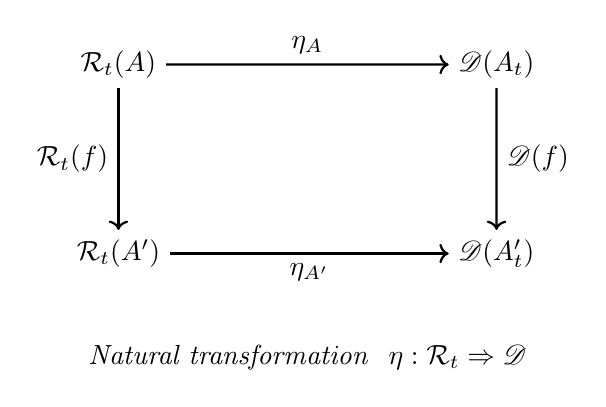
\begin{tikzpicture}[scale=1.2, every node/.style={font=\normalsize}]
			% Nodes
			\node (RtA) at (0,2) {${\mathcal{R}_t(A)}$};
			\node (RtA') at (0,0) {${\mathcal{R}_t(A')}$};
			\node (DA) at (4,2) {${\mathscr{D}(A_t)}$};
			\node (DA') at (4,0) {${\mathscr{D}(A_t')}$};
			
			% Arrows
			\draw[->, thick] (RtA) -- node[above] {$\eta_A$} (DA);
			\draw[->, thick] (RtA) -- node[left] {$\mathcal{R}_t(f)$} (RtA');
			\draw[->, thick] (DA) -- node[right] {$\mathscr{D}(f)$} (DA');
			\draw[->, thick] (RtA') -- node[below] {$\eta_{A'}$} (DA');
			
			% Label
			\node at (2,-1.1) {\textit{Natural transformation } $\eta: \mathcal{R}_t \Rightarrow \mathscr{D}$};
		\end{tikzpicture}
		\caption{Commutative diagram expressing the naturality of the defect tensor under RG flow.}
		\label{fig:defecttensorflow}
		
	\end{figure}
	
	\begin{example}{Some preliminary defect tensor details}{ex4}
		
		We formalize the renormalization group smoothing and defect identification as functors in the category \( \mathcal{C}_Q \) of liquid crystal configurations.
		
		\paragraph{RG flow as a functor.}
		Define a renormalization group functor:
		\[
		\mathcal{R}_t: \mathcal{C}_Q \to \mathcal{C}_Q, \quad (M, g, Q) \mapsto (M, g, Q_t),
		\]
		where \( Q_t(x) = \int_M K_t(x,y) Q(y) \, d\mathrm{vol}_g(y) \) is the smoothed field via heat kernel \( K_t \).
		
		\paragraph{Defect tensor as a functor.}
		Let the defect tensor functor, as in \cite{schimming2025defect}, be:
		\[
		\mathscr{D}: \mathcal{C}_Q \to \mathcal{C}_\rho, \quad Q \mapsto \rho(x) = \delta[Q(x) - Q_d] \cdot D(x),
		\]
		with
		\[
		D_{r\alpha}(x) = \varepsilon_{\alpha\mu\nu} \, \partial_i Q_{\mu\beta} \, \partial_j Q_{\nu\gamma} \, Q_{\beta\delta} Q_{\gamma\delta}.
		\]
		
		\paragraph{Naturality condition.}
		The following diagram commutes for any morphism \( f: A \to A' \in \mathcal{C}_Q \): [Fig. \ref{fig:defecttensorflow}]. This ensures functorial compatibility between RG smoothing and topological defect diagnostics.
		
		\paragraph{Spectral decomposition of the defect tensor.}
		We analyze \( D_{r\alpha} \in \mathbb{R}^{3 \times 3} \) as an antisymmetric matrix at each point \( x \). Define the matrix:
		\[
		D(x) = \left( D_{r\alpha}(x) \right), \quad D^T = -D.
		\]
		Then \( D \) has purely imaginary eigenvalues \( \{0, \pm i\lambda(x)\} \), where \( \lambda(x)^2 = -\tfrac{1}{2} \operatorname{Tr}(D^2(x)) \).
		
		The spectral norm:
		\[
		\|D(x)\|^2 = -\tfrac{1}{2} \operatorname{Tr}(D^2) = \sum_{\alpha, r} D_{r\alpha} D_{r\alpha},
		\]
		is a scalar field on \( M \) sharply peaked at disclination cores, thus serving as a defect magnitude field. This provides an invariant signature of topological structure under RG evolution.
		
	\end{example}
	
	
	
	\begin{remark}
		Because the torus has zero Euler characteristic, the ability to annihilate defects of opposite charge depends on geometric and energetic criteria, not topological obstructions. The categorical formulation separates these constraints cleanly, making the framework suitable for classification and computation.
	\end{remark}
	
	\begin{example}{Broad-strokes analysis of functorial RG flow from microscopic to mesoscopic scales}{ex:micromeso}
		
		Let \( A_{\mathrm{micro}} = (M, g, Q^{\mathrm{micro}}) \in \mathcal{C}_Q \) represent a microscopic configuration on a 3D ball \( M = B^3 \), with a high-resolution \( Q \)-tensor field that exhibits sharp disclination lines. Define the RG flow functor:
		\[
		\mathcal{R}_t: \mathcal{C}_Q \to \mathcal{C}_Q, \quad Q \mapsto Q_t = \int_M K_t(x, y) Q(y) \, d\mathrm{vol}_g(y),
		\]
		where \( K_t(x,y) \) is a heat kernel with scale \( \sqrt{t} \). Then define the mesoscopic object:
		\[
		A_{\mathrm{meso}} = \mathcal{R}_t(A_{\mathrm{micro}}) = (M, g, Q^{\mathrm{meso}} = Q_t).
		\]
		
		\paragraph{Defect tensor flow.}
		Apply the defect tensor functor \( \mathscr{D} \):
		\[
		\mathscr{D}(A) = \rho(x) = \delta[Q(x) - Q_d] \cdot D_{r\alpha}(x),
		\quad \text{with} \quad D_{r\alpha} = \varepsilon_{\alpha\mu\nu} \, \partial_i Q_{\mu\beta} \, \partial_j Q_{\nu\gamma} \, Q_{\beta\delta} Q_{\gamma\delta}.
		\]
		
		This gives topological current density fields \( \rho^{\mathrm{micro}} \) and \( \rho^{\mathrm{meso}} \) corresponding to sharp and smoothed disclination structures, respectively.
		
		\paragraph{Naturality of defect flow.}
		The RG transformation and defect projection commute under the natural transformation:
		\[
		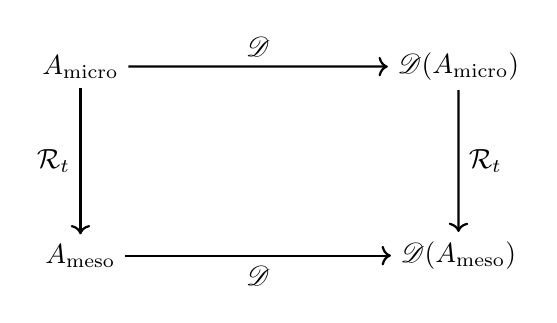
\begin{tikzpicture}[scale=1.2, baseline=(current bounding box.center)]
			\node (A) at (0,2) {$A_{\mathrm{micro}}$};
			\node (B) at (0,0) {$A_{\mathrm{meso}}$};
			\node (C) at (4,2) {$\mathscr{D}(A_{\mathrm{micro}})$};
			\node (D) at (4,0) {$\mathscr{D}(A_{\mathrm{meso}})$};
			
			\draw[->, thick] (A) -- node[left] {$\mathcal{R}_t$} (B);
			\draw[->, thick] (A) -- node[above] {$\mathscr{D}$} (C);
			\draw[->, thick] (B) -- node[below] {$\mathscr{D}$} (D);
			\draw[->, thick] (C) -- node[right] {$\mathcal{R}_t$} (D);
		\end{tikzpicture}
		\quad \Rightarrow \quad \eta: \mathcal{R}_t \Rightarrow \mathscr{D}.
		\]
		
		\paragraph{Interpretation.}
		This diagram expresses that disclination information propagates consistently under smoothing: the smoothed defect field \( \rho^{\mathrm{meso}} \) is equal (up to convolution) to the image of \( \rho^{\mathrm{micro}} \) under \( \mathcal{R}_t \). Thus:
		\[
		\mathscr{D}(Q_t) = \mathcal{R}_t(\mathscr{D}(Q)).
		\]
		
		\paragraph{Preliminary spectral diagnostics.}
		At each scale \( t \), the local spectrum of the antisymmetric defect tensor \( D(x) \in \mathfrak{so}(3) \) yields eigenvalues \( \{ 0, \pm i \lambda(x) \} \), with:
		\[
		\lambda(x)^2 = -\tfrac{1}{2} \operatorname{Tr}(D^2(x)).
		\]
		
	\end{example}
	
	\begin{example}{Spectral diagnostics under anchoring variation}{ex:anchoring}
		
		Let \( M = B^3 \subset \mathbb{R}^3 \) and consider a director field with anchoring tilt angle \( \theta_a \in [0, \pi/2] \), interpolating between:
		\begin{itemize}
			\item \( \theta_a = 0 \): homeotropic (normal anchoring),
			\item \( \theta_a = \pi/2 \): planar degenerate (tangential anchoring),
			\item \( \theta_a \in (0, \pi/2) \): tilted hybrid anchoring.
		\end{itemize}
		
		Define the director field:
		\[
		\mathbf{n}(x) = \cos \theta_a \, \hat{\mathbf{r}} + \sin \theta_a \, \hat{\mathbf{t}}(x),
		\]
		where \( \hat{\mathbf{r}} = \frac{\mathbf{x}}{\|\mathbf{x}\|} \), and \( \hat{\mathbf{t}}(x) = \frac{\hat{z} \times \mathbf{x}}{\|\hat{z} \times \mathbf{x}\|} \) is a local tangent vector. Let the uniaxial tensor field be:
		\[
		Q_{ij}(x) = S(r)\left(n_i n_j - \tfrac{1}{3} \delta_{ij}\right).
		\]
		
		The defect tensor is:
		\[
		D_{r\alpha} = \varepsilon_{\alpha\mu\nu} \, \partial_i Q_{\mu\beta} \, \partial_j Q_{\nu\gamma} \, Q_{\beta\delta} Q_{\gamma\delta}.
		\]
		
		\paragraph{Spectral norm.}
		The squared spectral norm is:
		\[
		\lambda(x)^2 = -\tfrac{1}{2} \operatorname{Tr}(D^2(x)) = \sum_{r,\alpha} D_{r\alpha}^2.
		\]
		
		Near the boundary \( r \to R \), radial derivatives vanish, and angular variation dominates. This yields the leading order estimate:
		\[
		\lambda^2(x) \approx \frac{C \cdot S^4}{r^4} \cdot \sin^2(2\theta_a),
		\]
		where \( C > 0 \) depends on the angular configuration of \( \hat{\mathbf{t}} \).
		
			\begin{center}
			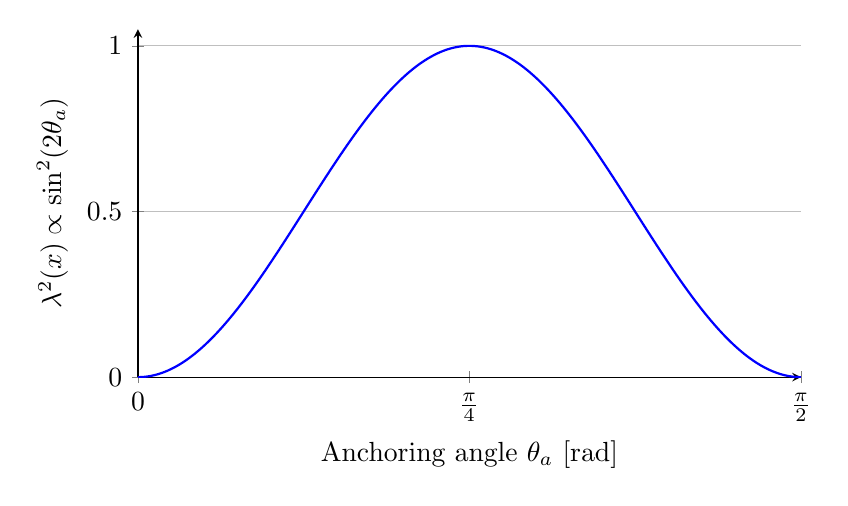
\begin{tikzpicture}
				\begin{axis}[
					width=10cm,
					height=6cm,
					xlabel={Anchoring angle $\theta_a$ [rad]},
					ylabel={$\lambda^2(x) \propto \sin^2(2\theta_a)$},
					xmin=0, xmax=1.571,
					ymin=0, ymax=1.05,
					xtick={0, 0.785, 1.571},
					xticklabels={$0$, $\frac{\pi}{4}$, $\frac{\pi}{2}$},
					ymajorgrids=true,
					axis lines=left,
					domain=0:1.571,
					samples=200,
					]
					\addplot[thick, blue] {sin(deg(2*x))^2};
				\end{axis}
			\end{tikzpicture}
		\end{center}
		
		\paragraph{Categorical interpretation.}
		Define a functor \( \lambda: \mathcal{C}_Q \to \mathcal{C}_{\mathrm{scal}} \) extracting the spectral scalar field:
		\[
		\lambda^2 \circ \mathcal{R}_t (A_{\theta_a}) = \text{RG-evolved defect norm}.
		\]
		Then the function \( \theta_a \mapsto \lambda^2 \) classifies anchoring effects on topological activity.
		
		
		\paragraph{Conclusion.}
		The spectral norm of the defect tensor peaks at \( \theta_a = \pi/4 \), corresponding to maximally tilted anchoring. This invariant classifies how strongly defects are encoded in the \( Q \)-tensor field under geometrically varying boundary conditions.
		
	\end{example}
	



	
	

	
	
	\section{Working End (No conclusion yet)}
	
	We are developing a multiscale categorical field theory for liquid crystals that integrates renormalization group flows with the compositional structure of category theory. By interpreting RG transformations as functors, we preserve the informational content across scales and link microscopic details with macroscopic phenomena. Our framework draws on classical foundations \cite{maclane1971categories, degennes1993physics} and modern perspectives from topological and higher gauge theories [\cite{atiyah1988topological, segal2004definition, baez2007higher, freed1995chern}]. Furthermore, connections with functional programming paradigms [\cite{hudak1989conception}] and categorical semantics in quantum protocols [\cite{abramsky2004categorical, selinger2007dagger}] underscore the broad applicability of these ideas.
	
	This work opens new avenues for research into the interplay between geometry, topology, and stochastic dynamics in liquid crystals, and more broadly, in complex physical systems.
	
	\newpage
	\bibliographystyle{apalike}
	\bibliography{references}
	
\end{document}
